\setcounter{page}{1}
\clubpenalty=10000 
\widowpenalty=10000
%%%%%%%%%%%%%%%%%%%%%%%%%%%%%%%%%%%%%%%%
%      Шапка экспертной организации  
%%%%%%%%%%%%%%%%%%%%%%%%%%%%%%%%%%%%%%%%
%
%%%%%%%%%%%%%%%%%%%%%%%%%%%%%%%%%%%%%%%%%
%
%   Экспертная организация ООО Южнорегиональная экспертная группа
%
%%%%%%%%%%%%%%%%%%%%%%%%%%%%%%%%%%%%%%%%%
\noindent %\qrcode[height=21mm]{\NomerDoc от \окончено }  %%% Добавлен QR-Code
\begin{pspicture}(21mm,21mm)
\obeylines
\psbarcode{%
	%\NomerDoc от \окончено
	BEGIN:VCARD^^J
	VERSION:4.0^^J
	%N:Мраморнов; Александр; Вчеславович^^J
	FN:Александр Мраморнов^^J
%	ORG:IP Alexandr Mramornov^^J
	TITLE: эксперт
	ORG: ИП
	URL:http://www.yourexp.ru^^J
	EMAIL:4516611@gmail.com^^J
	TEL:+7-918-451-6611^^J
	ADR:г. Краснодар, с/т № 2 А/О «Югтекс», ул. Зеленая, 472^^J
	END:VCARD
}{width=1.0 height=1.0}{qrcode}%
\end{pspicture}
\begin{center}
	\normalsize\textbf{$\cdots$\\[-1.5mm] <<$\cdots$>> \\[-5mm]}
	%  
	\noindent\rule{\textwidth}{1pt}\\[-6mm]  % Горизонтальная линия
	% \line(1,0){460}% (1,0) -горизонтальная линия, и (0,1) - вертикальная 
\end{center}

\begin{center}
	\begin{footnotesize}\setstretch{0.3}
		%	\small\textbf\setlength   	%\raisebox{5mm}
		\vspace{-3.5mm}$\cdots$\\[0mm]
		Телефон: \quad $\cdots$, e-mail:\quad $\cdots$\\ [-2mm]{$\cdots$\quad$\cdots$}
	\end{footnotesize}	\\[10mm]
\end{center}


\begin{flushright}
	%Краснодар,
	$\cdots$, 2020    \\[8mm]
\end{flushright}
\begin{center}
	\LARGE\textbf{ ЗАКЛЮЧЕНИЕ ЭКСПЕРТА}
	\bigskip\\[0mm]
	%	{\normnumxtbf{\NomerDoc}}	}{den}
\end{center}
\par
\vspace{-3mm}\noindent по гражданскому делу \delonum \, по иску \isk \\[0mm]

%\raggedright 
%\def\hrf#1{\hbox to#1{\hrulefill}}
\noindent \textbf{№ $\cdots$}\hfill           \textbf{\окончено}\\%[2mm]
%Приостановлено\hfill      \datastop\\
%Возобновлено\hfill          \datarestart\\
%Окончено\hfill                \dataend\\%[4mm]

\noindent\parbox[l][16mm]{16.5cm}
{\def\hrf#1{\hbox to#1{\hrulefill}}
	\noindent Начато\hfill            \datastart\\%[2mm]
	%	Приостановлено\hfill      \datastop\\
	%	Возобновлено\hfill          \datarestart\\
	Окончено\hfill                \окончено\\%[4mm]
}
\relax

\datastart г. ~в {\small $\cdots$} \,  при определении  \, \sud  \,  от \, \dataopr \, о назначении \opr \, по гражданскому делу \delonum \, поступили:

\begin{enumerate}\setlist{nolistsep}\item  Материалы гражданского дела \delonum \\[-2mm]
	%	\item  
\end{enumerate}Экспертиза произведена экспертом  $\cdots$  % Шапка организации ООО ЮРЕКСГРУП
%
%%   вопросы экспертизы
\subsection{Вопросы экспертизы}
%Заказчик поручает, а Исполнитель принимает на себя обязательство выполнить Заказчику  комплекс работ в виде автотехнических исследований автомобиля Mazda 6, VIN RUMGJ52\-6802007133 (дата начала гарантии 07.05.2018 г.), по следующим вопросам:
\begin{enumerate}
	\item  <<Связано ли повреждение панели рамки радиатора слева и брызговика с лонжероном переднего левого автомобиля ВАЗ 21099 с указанным ДТП?>>	
\end{enumerate}

\addcontentsline{toc}{section}{Использованные нормативы и источники информации}
%
%\left( \addcontentsline{toc}{section}{Использованные нормативы и источники информации}

\subsection{Использованные нормативы и источники информации}
%
\begin{enumerate}
%	
%\vspace{-10mm}
%
%\item
%Федеральный закон от 31 мая 2001 г. N 73-ФЗ \emph{О государственной судебно-экспертной деятельности в Российской Федерации} 
%
%\item
%Федеральный закон от 25.04.2002 N 40-ФЗ \emph{Об обязательном страховании гражданской ответственности владельцев транспортных средств} // Собрание законодательства РФ  06.05.2002, N 18, ст. 1720
%
%\item
%Федеральный закон от 28 марта 2017 г. N 49-ФЗ \emph{О внесении изменений в Федеральный закон "Об обязательном страховании гражданской ответственности владельцев транспортных средств} // Российская газета - Федеральный выпуск №7234 (68)
%
%
%
\item 
Махнин\,Е.\,Л., Новоселецкий\, И.\,Н., Федотов\, С.\,В. \emph{Методические рекомендации по проведению судебных автотехнических экспертиз и исследований колесных транспортных средств в целях определения размера ущерба, стоимости восстановительного ремонта и оценки} // --М.: ФБУ РФЦСЭ при Минюсте России, 2018.-326 с.  ISBN 978-5-91133-185-6
%
%\item  «Исследование автомототранспортных средств в целях определения стоимости восстановительного ремонта и оценки» (Методические рекомендации для судебных экспертов, утверждено  научно-методическим советом РФЦСЭ 13 марта 2013 г., протокол №35.), Минюст России, 20013г.
%%
%\item  Судебная автотехническая экспертиза. Институт повышения квалификации Российского Федерального Центра Судебной Экспертизы, М. 2007.
%
%\item
%Положение Банка России от 19 сентября 2014 года № 432-П \emph{О единой методике определения размера расходов на восстановительный ремонт в отношении повреждённого транспортного средства} // Вестник банка России, № 93 (1571). Нормативные акты и оперативная информация
%Центрального банка Российской Федерации. Москва, 2014
%
%\item
%Положение ЦБ РФ от 19 сентября 2014 года №433-П \emph{О правилах проведения независимой технической экспертизы транспортного средства} // Вестник банка России, № 93 (1571). Нормативные акты и оперативная информация Центрального банка Российской Федерации. Москва, 2014
%
\item ГОСТ 58197-2018 \emph{Порядок проведения экспертизы качества автомототранспортных средств}
\item ГОСТ 7593-80 \emph{Покрытия лакокрасочные грузовых автомобилей. Технические требования}
\item ГОСТ 9.414-2012 \emph{Покрытия лакокрасочные. Метод оценки внешнего вида}
\item ГОСТ Р 54586-2011 \emph{Материалы лакокрасочные. Метод определения твёрдости покрытия по 	карандашу}
\item ГОСТ Р 51694-2000 \emph{Материалы лакокрасочные. Определение толщины покрытия}
\item ГОСТ 31149—2014 \emph{Материалы лакокрасочные. Определение адгезии методом решетчатого  надреза}
\item ГОСТ 9.407-2017 \emph{Единая система защиты от коррозии и старения} ПОКРЫТИЯ ЛАКОКРАСОЧНЫЕ. \emph {Термины и определения}
\item ГОСТ 9.407-2015 \emph{Единая система защиты от коррозии и старения} ПОКРЫТИЯ ЛАКОКРАСОЧНЫЕ. \emph {Метод оценки внешнего вида}
\item ГОСТ 857-1-2009 \emph{Сварка и родственные процессы}
%\item ГОСТ 15878-79  \emph{Контактная сварка. Соединения сварные. Конструктивные элементы и размеры}
%\item ГОСТ 23518-79 \emph{Дуговая сварка в защитных газах. Соединения сварные под острыми и тупыми углами. Основные типы, конструктивные элементы и размеры}
%
%\item
%ПОТ РМ-027-2003  \emph{Межотраслевые правила по охране труда на автомобильном транспорте} //
%Спб.: ЦОТПБСП, 2003. - 200 с.  ISBN 5-326-00140-3
%
%\item ТУ 017207-255-00232934-2014 \emph{Кузова автомобилей LADA. Технические требования при приемке в ремонт, ремонте и выпуске из ремонта предприятиями дилерской сети ОАО "АВТОВАЗ"}//  ОАО НВП "ИТЦ АВТО", 2014
%
%\item В.Л. Смирнов, Ю.С. Прохоров, В.С. Боюр и др. \emph{Автомобили ВАЗ. Кузова. Технология ремонта, окраски и  антикоррозионной защиты. Часть II}// -Н.Новгород: АТИС, 2001.-241с.
%
%\item ГОСТ 27.002-2015  \emph{«Надежность в технике. Термины и определения» }
%
%\item ГОСТ 2.610-2006 \emph{"Единая система конструкторской документации (ЕСКД). Правила выполнения эксплуатационных документов"}
%
%\bibitem{ca:x}
%Хусаинов\, А.\,Ш. \emph{Теория автомобиля: конспект лекций } //
%А.\,Ш.\,Хусаинов, В.\,В.\,Селифонов. – Ульяновсk: УлГТУ, 2008. – 121 с.
% 
\item \emph{Судебная автотехническая экспертиза} Институт повышения квалификации Российского Федерального Центра Судебной Экспертизы, М. 2007.
%
%\item
%\emph{Марочник сталей и сплавов} Под редакцией Зубченко А.С. — М.:
%Машиностроение, 2003 г
\item \emph Л.П. Шестопалова, Т.Е. Лихачева {Методы исследования материалов и деталей машин при проведении автотехнической экспертизы}// учеб. пособие /
. – М.: МАДИ, 2017. – 180 с.
%
%\item  Кутателадзе С.С. \emph{Основы теории теплообмена}. – М.: Атомиздат, 1979. – 416с.
%
%\item \emph{Двигатели внутреннего сгорания. Теория поршневых и комбинированных двигателей}. – Под ред. С. Орлина,  М .Круглова. М.: Машиностроение, 1983.- 372с.
%
%\item
%Корухов\,Ю.\,Г., Замиховский\, М.\,И. \emph {Криминалистическая фотография и видеозапись для экспертов-автотехников} // Практическое пособие М.: ИПК РФЦСЭ при МЮ РФ, 2006г.
%
\item
Чава\,И.\,И. \emph {Судебная автотехническая экспертиза} // Учебно-методическое пособие для  экспертов,    судей, следователей, дознавателей и адвокатов. НП «Судэкс», Москва, 2014.
%
%\item
%Краснопевцев\,Б.,В. \emph{Фотограмметрия} // Учебное пособие. МИИГАиК, 2008.
%
%\item Хрулев\,А.\,Э. \emph{Ремонт двигателей зарубежных автомобилей} // Производственно-практ. издание --М.: Издательство "За рулем", 1999. --440 с., ил., табл.  ISBN 5-85907-084-5
%
%\item \emph{Исследование транспортных средств в целях определения стоимости восстановительного ремонта и оценки: курс лекций} // под общ. ред. д-ра юрид. наук, профессора С.А. Смирновой; Министерство юстиции Российской Федерации, Федеральное бюджетное учреждение Рос. Федер. центр судеб экспертизы. - М.: ФБУ РФЦСЭ при Минюсте России, 2017. - 286 с.
%
%\item  \emph{Технологическое руководство «Приемка, ремонт и выпуск из ремонта кузовов легковых автомобилей предприятиями автотехобслуживания»} РД 37.009.024-92
%
%\item Карасев А.\,И. \emph{Теория вероятностей и математическая статистика} : учебник. М.: Статистика, 1979. 279 с.
%
%\item А.\,П. Ковалев, А.\,А. Кушель, И.\,В. Королев, П.\,В. Фадеев	\emph{Практика оценки стоимости машин и оборудования} : учебник //  ; под ред. М. А. Федотовой. М. : Финансы и статистика, 2005. 272 с.
%\item
%Утакаева И.Х. \emph{Применение пакета статистического анализа Python для анализа данных автомобильного рынка}// Вестник Алтайской академии экономики и права. – 2019. – № 2-2. – С. 346-351; 
%
%\item Макушев\,Ю.П., Иванов\,А.Л. \emph{Упрощенный расчет турбокомпрессора для двигателя внутреннего сгорания} // Сибирская государственная автомобильно-дорожная академия, г. Омск, Омский научный вестник № 4 (73), 2008
%
%\item Герт Хак \emph{Турбодвигатели и компрессоры} // Справ. пособие : Пер. с нем., Лангкабель. - М. : АСТ : Астрель, 2003. - 350 с. : ил., 25 см. ISBN 5170193777
%
%\item Повреждения поршней // Группа Motorservice, Kolbenschmidt Pierburg, www.ms-motorservice.com
%
%\item 	\emph{Повреждения подшипников скольжения}. Kolbenschmidt / MS Motorservice International Gmbh
%
%\item Хрулев А.Э., Кротов М.В. \emph{Влияние неисправностей в системе смазки на характер повреждения подшипников ДВС}. Научно-технический журнал "Двигатели внутреннего сгорания" №1/2018, DOI: 10.20998/0419-8719.2018.1.13
%
%\item  \emph{Анализ и предотвращение отказов подшипников}. https://access.cummins.com
%
%\item 	\emph{Руководство по замене вкладышей и устранению повреждений вкладышей}. Federal-Mogul Corportion/ General Distribution Centre, Belgium
%
\item
Автомобильный справочник //  Пер. с англ.  -- 2-е изд., перераб. и доп. --М.:ЗАО "КЖИ "За рулем", 2004. --992 с.: ил.  ISBN 5-85907-327-5
%
%\item
%Справочник физических свойств материалов //  www.matweb.com   by MatWeb, LLC
%\item
%Суворов\,Ю.\,Б. \emph{Судебная дорожно-транспортная экспертиза} // М.\,«Экзамен»
%
\item
Чалкин\,А.\,В.  \emph{Осмотр, фиксация и моделирование механизма образования внешних повреждений автомобилей с использованием их масштабных изображений} / А.\,В. Чалкин, А.\,Л. Пушнов, В.\,В. Чубченко // Учебное пособие -- М.:ВНКЦ МВД СССР 1991г.
%
%URL: https://vaael.ru/ru/article/view?id=334
%
%\bibitem{torm}
%Булгаков \,Н.\,А.  \emph{Исследование динамики торможения автомобиля} / Н.\,А. Булгаков, А.Б. Гредескул, С.\,И Ломака // Научное сообщение № 18.- Харьков: Изд-во Харьковского госуниверситета, 1962. - 36 с.
%
%\bibitem{prich}
%Бутырин\, А.\,Ю. \emph{Характеристика обстоятельств, имеющих значение при проведении казуальных автотехнических и строительно-технических судебно-экспертных исследований} / А.\,Ю. Бутырин, Д.\.С. Дубровский, Е.\,А. Холина, И.\,И. Чава // Юридический журнал № 4,- М.:  2010

\item Петер фон ден Керкхофф, Гельмут Хааген. \emph{«Каталог повреждений лакокрасочных покрытий»}//-- М., Издательский дом Третий Рим, 2004.
\item Технические бюллетени авторемонтных материалов CarSYSTEM, \url{https://www.carsystem.org}, \url{http://www.carsystem.ru}
%
\item Шпатлевки полиэфирные «Novol». Технические карты. \url{http://professional.novol.pl/ru/}
%\item
%\emph{Сервис по автоматической расшифровке VIN номеров – AudaVIN} // Audatex
%
\item
\emph{Методика окраски и расчета стоимости лакокрасочных материалов для проведения окраски транспортных средств   AZT}// http://azt-automotive.com,   http://www.schwacke.ru/\-ereonline.htm

%\item \emph{CRASH 3 Technical Manual}. National Highway Traffic Safety Administration, \url{www-nass.nhtsa.gov}
%%
%\item
%\emph{Информационно-справочная система по ремонту и сервисному обслуживанию автомобилей Autodata}// Autodata online, лицензионный код GA0288799, Autodata Group Ltd, Великобритания. Дистрибьютор в России ЗАО «Легион-Автодата», www.autodata.ru, www.autodata-online.ru
%
\item
\emph{Специализированное программное обеспечение для расчета стоимости  восстановительного ремонта, содержащее нормативы трудоемкости работ, регламентируемые изготовителями транспортного средства}//   AudaPadWeb, лицензионное соглашение № AS/APW-658  RU-P-409-409435

%\item
%\emph{Электронный каталог деталей автомобилей}// www.elcats.ru
%
\item
\emph{Электронный каталог деталей автомобилей}// \url{http://zavod-nn.ru/}

%\item
%\emph{Электронный каталог деталей автомобилей}//http://lada-original.ru/catalog/
%%
%\item  \emph{Электронная база данных РСА  средней стоимости запасных частей и нормо-часа работ} //http://prices.autoins.ru/spares/
%%
%\item
%\emph{Цены оригинальных деталей на автомобили Мерседес Бенц}https://partsprice.mercedes-benz.ru/?owda=misc
%%
%\item Интернет-ресурсы:\\
%\url{emex.ru}\\
%\url{exist.ru}\\
%\url{autopiter.ru}\\
%\url{autostels.ru}\\
%\url{autokorea22.ru}\\
%\url{chevrolet-daewoo-parts.ru}
%
%Аверьянова Т.В., Белкин Р.С., Корухов Ю.Г., Россинская Е.Р. Криминалистика. – М.: Норма, 2003.
%Акимов С.В. Электрооборудование автомобилей: Учебник для вузов/ С.В.Акимов, Ю.П.Чижков./ М.:Аист Принт Изд-во ООО, 2003.
%Андрианов Ю.В. Как оценить и возместить ущерб от дорожно-транспортного происшествия. - М.: «Дело», 2002.
%Арбитражный процессуальный кодекс Российской Федерации.
%Арсеньев В.Д. Соотношение понятий предмета и объекта в судебной экспертизе // Проблемы теории судебной экспертизы: Сб. науч. тр. ВНИИСЭ. – М., вып. 44, 1980.
%Бабков В.Ф. Автомобильные дороги. – М.: Транспорт, 1983.
%Бабков В.Ф. Дорожные условия и безопасность движения. – М.: Транспорт, 1993.
%Байэтт Р., Уоттс Р. Расследование дорожно-транспортных происшествий / Пер. с англ. – М.: Транспорт, 1983.
%Белкин Р.С. Курс криминалистики. – М.: Закон и право, 2001.
%Бирюков Б.М.. Интернет-справочник автомобилиста 2001: Автосправка; Маркировка автомобилей; Автомобильные каталоги и базы данных; Продажа и покупка автомобилей; Запчасти к автомобилям; Тюнинг, ремонт и ТО автомоб. – М.:ТИД КОНТИНЕНТ-Пресс, 2001.
%Боровских Ю.И. Техническое обслуживание и ремонт автомобилей. – М.: Высшая школа, 1988.
%Винберг А.И., Мирский Д.Я., Ростов М.Н. Гносеологический, информационный и процессуальный аспекты учения об объекте судебной экспертизы // Вопросы теории и практики судебной экспертизы: Сб. науч. тр. ВНИИСЭ. – М., 1983.
%Возможности производства судебной экспертизы в государственных судебно-экспертных учреждениях Минюста России – М., Антидор, 2004.
%Гаврилов К.Л. Диагностика электрооборудования автомобилей: Практическое руководство /Константин Гаврилов./ М.:НЦ ЭНАС Изд-во ЗАО, 2001.
%Гражданский процессуальный кодекс Российской Федерации.
%Грановский Г.Л., Поляков В.З., Майлис Н.П. Математическое моделирование в производстве трасологических экспертиз // Моделирование при производстве трасологических экспертиз: Сб. науч. тр. ВНИИСЭ. – М., вып. 49, 1981.
%Грановский Г.Л., Поляков В.З., Майлис Н.П. Математическое моделирование в производстве трасологических экспертиз // Моделирование при производстве трасологических экспертиз: Сб. науч. тр. ВНИИСЭ. – М., вып. 49, 1981.
%Григорян В.Г. Определение наличия (отсутствия) у водителя ТС технической возможности предотвратить наезд на пешехода // Проблемы судебной автотехнической экспертизы. – М. ВНИИСЭ, 1988.
%Григорян В.Г. Применение в экспертной практике параметров торможения автотранспортных средств: Методические рекомендации. – М.: РФЦСЭ, 1995.
%Дефекты автомобильных шин. Каталог. – М.: НИИШП, 2000.
%Дорожная терминология: Справочник / Под ред. М.И. Вейцмана. – М.: Транспорт, 1985.
%Жилинский Г.В., Суворов Ю.Б. Особенности исследования технического состояния транспортных средств, участвовавших в ДТП // Автомобильный транспорт. – 1986. – № 9.
%Жулев В.И. Предупреждение дорожно-транспортных происшествий. – М.: Юридическая литература, 1989.
%Замиховский М.И. и др. Определение характера движения ТС по следам колес: Методическое письмо. – М.: ВНИИСЭ, 1993.
%Замиховский М.И. и др. Экспертное исследование следов на ТС, возникших при ДТП: Метод. письмо. – М.: ВНИИСЭ, 1994.
%Замиховский М.И. Экспертная реконструкция механизма ДТП по его следам: Автореф. канд. дис. – М.: ВНИИСЭ, 1991.
%Замиховский М.И., Самарина Т.М. Комплексное изучение следов в целях идентификации человека, находившегося на месте водителя в момент ДТП // Экспертная техника. – М.: ВНИИСЭ, 1990. – Вып.114.
%Зинин А.М., Майлис Н.П. Судебная экспертиза (учебник для вузов). – М., 2002.
%Идентификация легковых автомобилей. Европа, Азия, Америка. — М., 1999 — 2000.
%Иларионов В.А., Чернов В.И., Дадашев Ф.А. Расчет параметров маневра транспортных средств: Метод. письмо для экспертов. – М.: ВНИИСЭ, 1988.
%Исаев А.А., Иванова Н.Ю., Замиховский М.И. Трасологическое определение механизма наезда ТС на пешехода: Метод реком. – М.: ВННИСЭ, 1990.
%Исследование обстоятельств дорожно-транспортного происшествия», Чава И.И., Москва, 2007 г.
%Каталоги запасных частей автомобилей ЗАЗ, ВАЗ, АЗЛК и Иж, ГАЗ (легковые), ГАЗ (грузовые), УАЗ, ЗиЛ (грузовые), МАЗ, КамАЗ, КРАЗ, «Урал», автобусов РАФ, ЛИАЗ, ПАЗ, тракторов. — М.: 2000 «Прайс - Н».
%Классификация основных методов судебной экспертизы. – М.: ВНИИСЭ, 1982.
%Кодекс Российской Федерации об административных правонарушениях.
%Колдин В.Я., Полевой Н.С. Информационные процессы и структуры в криминалистике. – М.: МГУ, 1985.
%Колеса и шины: Краткий справочник: Выпуск 2/Сост. А.М.Ладыгина./ М.:Катера и Яхты Журнал ЗАО КП, 2003.
%Комментарий к законодательству о судебной экспертизе – М., Норма, 2004.
%Комментарий к Федеральному закону «О государственной судебно-экспертной деятельности в Российской Федерации». – М., Проспект, 2002.
%Корухов Ю.Г. Криминалистическая диагностика при расследовании преступлений. – М.: Норма, 1998.
%Корухов Ю.Г. Трасологическая диагностика: Метод пособ. – М.: ВНИИСЭ, 1983.
%Косенков А.А. Диагностика неисправностей автоматических коробок передач и трансмиссий – Ростов-на-Дону: Изд-во ЗАО НЦ ЭНАС, 2003.
%Косенков А.А. Устройство тормозных систем иномарок и отечественных автомобилей – Ростов-на-Дону: Изд-во ООО Аист Принт, 2003.
%Кренцель Р.Б. Применение в экспертной практике экспериментально-расчетных значений параметров легкости рулевого управления автомобилей: Метод. реком. – М.: ВНИИСЭ, 1993.
%Курзуков Н.И. Аккумуляторные батареи: Краткий справочник/Н.И.Курзуков, В.М.Ягнятинский./ 2003.
%Майлис Н.П. Судебная трасология. М.: Право и закон, 2003.
%Методические рекомендации по применению нормативных документов (актов) в автотехнической экспертизе. РФЦСЭ, 2004.
%Методические рекомендации: Установление признаков дифференциации и характеристик покрытий автомобильных дорог на месте дорожно-транспортных происшествий. – М.: РФЦСЭ при Минюсте России, 1995.
%Методическое руководство Определение стоимости, затрат на восстановление и утраты товарной стоимости автотранспортных средств. - СПб, СЗРЦСЭ Минюста России, РФЦСЭ при Минюсте России, 2001.
%Назначение и производство судебных экспертиз: Пособ. для следователей, судей и экспертов. – М.: Юридическая литература, 1988
%Назначение и производство судебных экспертиз: Пособие для следователей. /Под ред. Аринушкина Г.П., Шляхова А.Р. – М.: Юридическая литература, 1988.
%Немчинов М.В. Сцепные качества дорожных покрытий и безопасность движения автомобиля. – М.: Транспорт, 1985.
%Орлов Ю.К. Судебная экспертиза как средство доказывания в уголовном судопроизводстве – М., ИПК РФЦСЭ, 2005.
%Основные положения по допуску транспортных средств к эксплуатации и обязанности должностных лиц по обеспечению безопасности дорожного движения. – М.: Транспорт, 1995.
%Руководства изготовителей по эксплуатации транспортных средств.
%Сильянов В.В. Транспортно-эксплуатационные качества автомобильных дорог. – М.: Транспорт, 1984.
%Синельников Р.А., Лосавио С.К. Ремонт аварийных кузовов легковых автомобилей отечественного и иностранного производства. – М., Транспорт. 2001
%Сова Ф.П. Определение типов и моделей автотранспортных средств по следам шин: Учеб. пособ. – М.: ВШ МВД СССР, 1973.
%Современные возможности судебных экспертиз. Под ред. Ю.Г. Корухова – М., 2000.
%Солохин А.А. Судебно-медицинская экспертиза в случаях автомобильной травмы. – М., 1968.
%Соснин Д.А. Автотроника: Электрооборудование и системы бортовой автоматики современных легковых автомобилей: Учебное пособие - специалисту по ремонту и владельцам автомобилей/Дмитрий Соснин./ 2001.
%Справочник по месторасположению идентификационных номеров на легковых автомобилях. — М., 1996. — Вып. 2.
%Строительная, дорожная и специальная техника: Краткий справочник. А.А. Глазов и др. — М., 1998.
%Суворов Ю.Б. Анализ влияния эксплуатационных факторов системы ВАД для экспертного исследования причин ДТП // Теоретические и методические вопросы судебной экспертизы: Сб. науч. тр. ВНИИСЭ. – М., 1988.
%Суворов Ю.Б. Анализ влияния эксплуатационных факторов системы ВАД для экспертного исследования причин ДТП В сб. Теоретические и методические вопросы судебной экспертизы. – М.: ВНИИСЭ, 1988.
%Суворов Ю.Б. и др. Диагностическое исследование элементов автомобильных дорог, влияющих на безопасность дорожного движения (дорожных условий), на участках ДТП: Метод. пособ. для экспертов, следователей и судей. – М.: ВНИИСЭ, 1990.
%Суворов Ю.Б. Интерпретация и использование выводов экспертов по результатам производства экспертиз водителя и дороги. В сб. Вопросы теории и практики судебной экспертизы. – М.: ВНИИСЭ, 1990.
%Суворов Ю.Б. Комплексное экспертное исследование причин ДТП. Учет факторов системы ВАД при установлении непосредственных причин ДТП экспертом // Экспертная практика и новые методы исследования. – М.: ВНИИСЭ, 1993. – Вып. 9.
%Суворов Ю.Б. Новые виды, состояние и перспективы развития САТЭ // Проблемы судебной автотехнической экспертизы: Сб. науч. тр. ВНИИСЭ. – М., 1988.
%Суворов Ю.Б. Судебная дорожно-транспортная экспертиза. Судебно-экспертная оценка действий водителей и других лиц, ответственных за обеспечение безопасности дорожного движения на участках ДТП. Учебное пособие. – М.: Экзамен, 2003.
%Суворов Ю.Б. Судебная дорожно-транспортная экспертиза. Технико-юридический анализ причин дорожно-транспортных происшествий и причинно-действующих факторов. Учебное пособие. – М.: Приор, 1998.
%Суворов Ю.Б. Установление признаков дифференциации покрытий и характеристик автомобильных дорог на месте дорожно-транспортного происшествия: Метод. реком. – М.: РФЦСЭ, 1995.
%Суворов Ю.Б., Кочнев В.А. Методика и результаты экспериментального исследования влияния неравномерности снижения сцепных свойств дороги на параметры движения автомобиля при торможении. Инф. сборник. Экспертная практика и новые методы исследования. – М.: ВНИИСЭ, 1993. вып. 2.
%Суворов Ю.Б., Решетников Б.М., Кочнев В.А. Результаты экспериментального определения коэффициентов сцепления дорожных покрытий. В сб. «Экспертная техника», № 117. – М.: ВНИИСЭ, 1990.
%Судебная автотехническая экспертиза: Методическое пособие для экспертов-автотехников, следователей и судей /Под ред. В.А. Иларионова. – М.: ВНИИСЭ, 1980. – Ч. 2.
%Судебная дорожно-транспортная экспертиза». Экспертное исследование технического состояния дорог, дорожных условий на месте дорожно-транспортного происшествия, Суворов Ю.Б., Панина А.С., Москва, 2007 г.
%Транспортно-трасологическая экспертиза о дорожно-транспортных происшествиях», выпуск 1, методическое руководство для экспертов. Москва 2006 г.
%Транспортно-трасологическая экспертиза о дорожно-транспортных происшествиях», выпуск 2, методическое руководство для экспертов. Москва 2006 г.
%Транспортно-трасологическая экспертиза по делам о дорожно-транспортных происшествиях (Диагностические исследования): Метод. пособ. для экспертов, следователей и судей /Под редакцией Ю.Г. Корухова. – М.: ВНИИСЭ, 1988. – Вып. 1 и 2.
%Уголовно-процессуальный кодекс Российской Федерации.
%Федеральный закон от 31 мая 2001 г. № 73-ФЗ «О государственной судебно-экспертной деятельности в Российской Федерации».
%Фотография и видеозапись для экспертов-автотехников». Ю.Г.Корухов, Москва 2006 г.
%Чубченко А.П. и др. Отпечатки протекторов автотранспортных средств: Учеб. пособ. – М.: ВНИИ МВД СССР, 1987.
%Шляхов А.Р. Судебная экспертиза: организация и проведение. – М.: Юридическая литература, 1979.
%Эксперт // Руководство для экспертов органов внутренних дел и юстиции. Под ред. Т.В. Аверьяновой, В.Ф. Статкуса. – М., 2002.
%%
\end{enumerate}

%%%%%%%%%%%%%%%%%%%%%%%%%%%%%%%%%%%%%%%%%%%%%%%%%%%%%%%%%%%%%%%%%%%%%%%%%%%%%%%%%
\subsection{Технические средства}  %% Список не удалять!!!
\begin{itemize}
%
%%
%\item Диагностический сканер BOSH VCM II S/N 1324-88682639 c програмным обеспечением Mazda IDS - 115.02
%%\item   Диагностический сканер SDconnect   с программным обеспечением Xentry Diagnostics v19.11.3.1
%\item   Линейка масштабная магнитная с цветографической шкалой, 100мм
%%\item   Рулетка измерительная металлическая, 5м
%%\item  Универсальный стенд для измерения углов установки колес Hunter Engineering %ProAlign с программным инструментом регулировки схождения колес без блокировки руля %автомобиля WinToe
%\item 	Цифровой фотоаппарат Canon 760D s/n 143032001327 с объективом Canon EF-S 18-135, тип используемой памяти: Transcend,  32Gb
%\item  Специализированное программное обеспечение для расчёта стоимости  восстановительного ремонта, содержащее нормативы трудоёмкости работ, регламентируемые изготовителями транспортного средства     AudaPadWeb, лицензионное соглашение № AS/\- APW-658  RU-P-409-409435
\item Он-лайн программа моделирования кинематики подвески автомобиля // \url{http://www.vsusp.com/}
\item Он-лайн ресурс проверки метаданных цифровых изображений \url{http://exif.regex.info/exif.cgi}
\item  Программа обработки изображений с открытым исходным кодом ImageJ, разработанная для научных многомерных изображений.  Wayne Rasband (wa-yne@codon.nih.gov),
свободная лицензия GPL.
\item  ПЭВМ под управлением операционной системы Windows 10 с установленным набором макрорасширений LaTeX системы компьютерной вёрстки TeX, cвободная лицензия LaTeX Project Public License (LPPL). 
%	
\end{itemize}
%%%%%%%%%%%%%%%%%%%%%%%%%%%%%%%%%%%%%%%%%%%%%%%%%%%%%%%%%%%%%%%%%%%%%%%%%%%%%%%%%%%%%%%%%%%%%%%%%%%%%%
\subsection{Условные обозначения}

\begin{description}
%	 
%%\item[АВС] --антиблокировочная система
\item[АМТС] --автомототранспортное средство
%\item[ГРМ] -- газораспределительный механизм
\item[ДВС] --двигатель внутреннего сгорания
\item[ДТП] --дорожно--транспортное происшествие
\item[гос.\,рег.\,знак] --государственный регистрационный знак
\item[КТС] --колесное транспортное средство 
\item[ЛКП] --лакокрасочное покрытие
\item[л.д.] --лист дела
%%\item[Колесо турбины]  -- крыльчатка турбины
\item[ТС] --транспортное средство
%\item[ТK, ТКР] -- турбокомпрессор. Состоит из двух частей: турбины и компрессора, объединенных общим валом. Вал вращается в подшипниках, размещенных в центральном корпусе ТК
%\item[ЦПГ] -- цилиндро-поршневая группа
%\item[ЭБУ] --электронный блок управления
%%\item[FRAME] -- номер кузова транспортного средства, выпущенного для продажи на внутреннем рынке Японии и содержащий информацию производителя о транспортном средстве
%%\item[OBDII] -- On-board diagnostics. Протокол бортовой диагностики автомобиля
%%\item[SRS] -- Cистема пассивной защиты водителя и пассажиров
\item[VIN] --vehicle identification number, 17--значный идентификационный номер транспортного средства, соответствующий стандарту ISO 3779--2012.
%
\end{description}
%%%%%%%%%%%%%%%%%%%%%%%%%%%%%%%%%%%%%%%%%%%%%

\subsection{Методы исследования}

\begin{itemize}
\item  Органолептический метод – исследование и оценка качества объектов с помощью органов чувств
%\item 	Прямой измерительный метод – путем измерения размеров деталей специальными %измерительными приборами
\item Расчётный метод (косвенный измерительный метод) – путём расчётов различных параметров на основе результатов измерений и других данных
\item Экспертный метод (метод экспертной оценки) — совокупности операций по выбору комплекса или единичных характеристик объекта, определению их действительных значений и оценкой экспертом соответствия их установленным требованиям и/или технической информации
\item Графоаналитический метод  
\item Метод масштабного моделирования и проецирования
\end{itemize}
%%%%%%%%%%%%%%%%
%
\subsection{Термины и определения}
\begin{description}
	\item[Аварийные повреждения] --- повреждения, механизм образования которых определяется контактом с посторонними объектами, что привело к деформации или разрушению и к необходимости ремонта или замены составной части, или контактам с агрессивной средой, которая привела к необходимости ремонта (замены) составной части [1, часть II, п. 1.5].
	%	\item[Восстановительный ремонт]--- один из способов возмещения ущерба, состоящий в выполнении технологических операций ремонта КТС, действующий в сети торгово-сервисного обслуживания, созданной изготовителем этого КТС [1, часть II, п. 1.4].
%	\item[Годные остатки] --- работоспособные, имеющие остаточную стоимость детали (агрегаты, узлы) поврежденного автотранспортного средства, годные к дальнейшей эксплуатации, которые можно демонтировать с поврежденного автотранспортного средства и реализовать.
	\item[Дата исследования]--- дата, на которую проводятся расчеты и используются стоимостные данные КТС, запасных частей, материалов, нормо-часа ремонтных работ [1, часть II, п. 1.5].
	\item[Линия удара]--- линия, определяемая направлением вектора равнодействующего импульса сил, возникающих при контакте ТС при столкновении до прекращения взаимного внедрения деформирующихся при ударе частей. Положением линии удара на ТС определяются направление и величина момента импульса сил, возникающих при ударе, и, следовательно, направлением и интенсивность разворота ТС относительно центра масс после столкновения.  
	\item[Моделирование]--- исследование каких-либо явлений, процессов или систем объектов путем построения и изучения их моделей.
	\item[Морфологические признаки]--- признаки, отображающие внешнее и внутреннее строение объекта
	\item[Срок эксплуатации КТС]--- период времени от даты изготовления (даты выпуска) КТС, до даты оценки (исследования), определяемой условиями задачи исследования (независимо от даты его регистрации и начала использования по назначению (эксплуатации)).
\end{description}
%%%%%%%%%%%%%%%%%%%%%%%
\subsection{Исходные данные и объекты исследования}

19.07.2016 г.в 13 час.  42 мин. в г. Белореченске по ул. Красная, 66 водитель Терехов А.В., управляя автомобилем Renault, г/н Е431НЕ33 перед началом движения не предоставил преимущество и допустил столкновение с автомобилем \тс\, регистрационный знак \грз\, под управлением водителя Шамояна Р.О.  
\par Для производства исследования представлено:
\begin{enumerate}
\item материалы гражданского дела № \delonum, \, в том числе:
\begin{itemize}
	\item Копия акта осмотра № 6164 транспортного средства \тс\, составленного 29.07.2016 г.  специалистом  компании "РАНЭ" 
	\item Копия акта осмотра № 295 от 19 июля 2016 г., составленного индивидуальным предпринимателем Новиковым Олегом Николаевичем
	\item Копия свидетельства о регистрации ТС 23 38 № 793117
	\end{itemize}
\item Электронные копии цифровых фотоснимков поврежденного автомобиля \тс\, VIN \vin\, предоставленные в  количестве 16 файлов формата .jpg с сохраненными техническими данными EXIF, выполненные 19.07.2016 г. цифровым фотоаппаратом Сanon PowerShot SX150 IS 
\end{enumerate}

\subsection{Ранее по материалам дела выполнено}

\noindent Судебная автотехническая экспертиза, выполненная  экспертом Дереберя Н.В.\\
Повторная судебная автотехническая экспертиза, выполненная экспертом Алифиренко В.В.

\section{Исследование}
%
Установление связи между повреждениями автомобиля и заявленными событиями доро\-жно-транспортного происшествия есть вопрос  исследования   взаимосвязи между повреждением и механизмом, вызвавшим это повреждение. Разрешение поставленного вопроса предполагает исследование механизма происшествия с точки зрения анализа характера деформаций и причин образования повреждений компонентов транспортного средства.	В транспортной трасологии различают первичные следы -- следы, возникшие в процессе первичного, начального контакта транспортных средств между собой или транспортных средств с различными преградами, и вторичные следы-- следы, появившиеся в  процессе дальнейшего смещения и деформации вступивших в следовое взаимодействие объектов. Таким образом, если рассматривать объемный след в виде деформации, то различаются первичные деформации, характеризующиеся наличием признаков непосредственного контакта деталей и частей транспортных средств,  и вторичные деформации, характеризующиеся отсутствием признаков непосредственного контакта деталей и  частей транспортных средств. Вторичные деформации являются следствием первичных, контактных деформаций. Детали изменяют свою форму под воздействием сил и моментов, возникающих в случае контактных деформаций по законам механики и сопротивления материалов. Такие деформации могут располагаться на удалении от места непосредственного контакта воздействием силы удара, распространяющейся по деталям несущей конструкции кузова автомобиля.
 

 Из постановления об административном правонарушении и справки о дорожно-транс\-портном происшествии следует, что в результате столкновения левая часть автомобиля \тс\, взаимодействовала с передним бампером автомобиля 
 \tcb.
 
   В процессе следового взаимодействия контактирующие поверхности \тс \, в составе левого зеркала заднего вида, переднего левого крыла, передней левой двери деформирующим воздействием бампера переднего автомобиля \tcb\, получили повреждения в направлении спереди назад и слева направо.  Графо-аналитическим методом исследования фотоизображений  повреждений автомобиля \тс \, установлено, что повреждения левой стороны кузова автомобиля  содержат признаки динамического и статического деформирующих воздействий, в совокупности не противоречащие заявленному механизму дорожно-транспортного происшествия.
   
\begin{figure}[h!]\centering
	\parbox[t]{0.49\textwidth}
	{\centering
		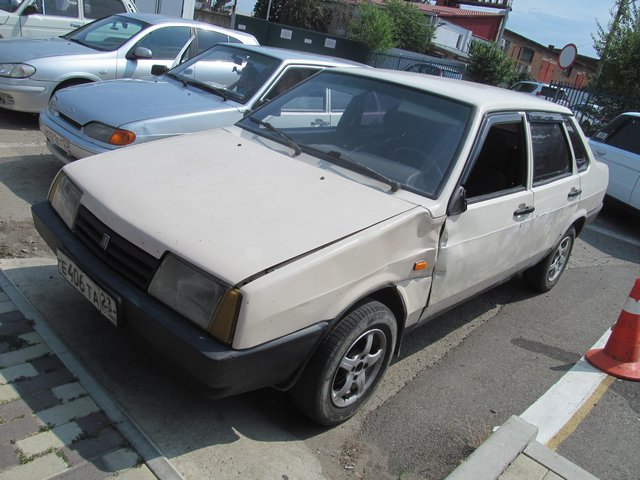
\includegraphics[width=.49\textwidth]{images/tc1}
		\caption{\footnotesize {Поврежденный в исследуемом ДТП автомобиль \тс,\, вид спереди слева}}
		\label{ris:images/b3}}
	\hfil \hfil
	\parbox[t]{0.49\textwidth}
	{\centering
		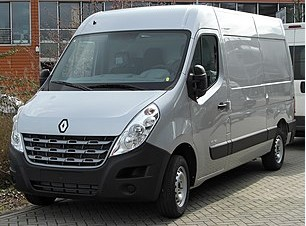
\includegraphics[width=.49\textwidth]{images/tb1}
		\caption{\footnotesize {Автомобиль, аналогичный автомобилю второго участника ДТП \tcb}}
		\label{ris:images/b4}}
\end{figure}



\subsection{Исследование транспортного средства}
%
С момента повреждения автомобиля до момента настоящего исследования прошел значительный период времени (более трех лет). Исходя из имеющихся в распоряжении эксперта изображений автомобиля, на момент ДТП, \датадтп\, на кузове автомобиля, преимущественно в нижней части, присутствовали  очаги коррозионных повреждений. Коррозия - физико-химическое или химическое взаимодействие между металлом и средой,  самопроизвольный окислительно-восстановительный процесс разрушения металлов и сплавов вследствие взаимодействия с окружающей средой,   необратимо усиливающихся с течением времени.  Ретроспективный характер исследования объективно не позволяет произвести натурное исследование автомобиля в том состоянии, в котором  автомобиль находился сразу  после заявленного ДТП.  На основании изложенного, исследование автомобиля \тс\, VIN \вин\, производилось экспертом по предоставленным электронным копиям цифровых фотоснимков. Представленные фотоснимки удовлетворительного качества и содержат необходимую и достаточную информации для производства экспертизы.


\begin{figure}[!h]\centering
	\parbox[t]{0.49\textwidth}
	{\centering
		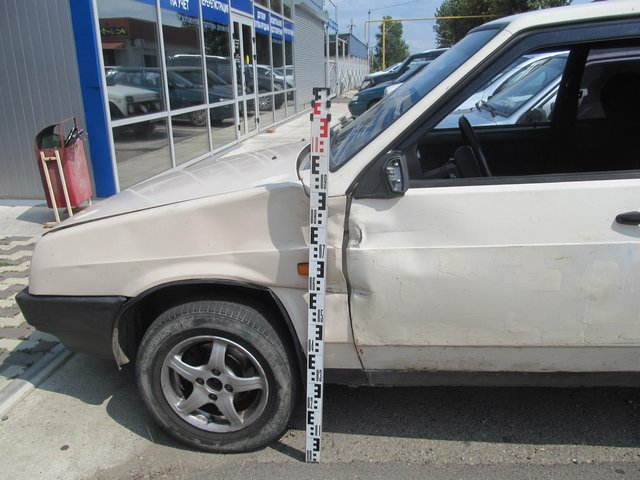
\includegraphics[width=.49\textwidth]{images/tc2}
		\caption{\footnotesize {Обзорный снимок поврежденной области исследуемого автомобиля }}
		\label{ris:images/tc2}}
	\hfil \hfil
	\parbox[t]{0.49\textwidth}
	{\centering
		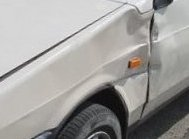
\includegraphics[width=.49\textwidth]{images/tc3}
		\caption{\footnotesize {Масштабное изображение  поврежденной области кузова исследуемого автомобиля}}
		\label{ris:images/tc3}}
	
\end{figure}



\begin{figure}[!h]\centering
	\parbox[t]{0.49\textwidth}
	{\centering
		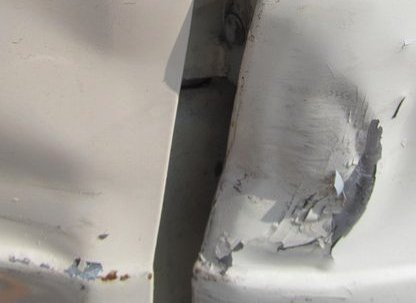
\includegraphics[width=.49\textwidth]{images/tc8}
		\caption{\footnotesize {Повреждение левой передней двери }}
		\label{ris:images/tc8}}
	\hfil \hfil
	\parbox[t]{0.49\textwidth}
	{\centering
		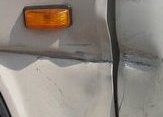
\includegraphics[width=.49\textwidth]{images/tc9}
		\caption{\footnotesize {Повреждение левого переднего крыла}}
		\label{ris:images/tc9}}
	
\end{figure}

Представленные  изображения первичных повреждений левой передней стороны автомобиля \тс\,,  получены в результате заявленного ДТП \датадтп.  Из материалов дела известно, что оспариваемыми  страховой компанией повреждениями являются повреждения    панели рамки рамки радиатора слева и  брызговика с лонжероном переднего левого, Рис. \ref{ris:images/tc5}, Рис. \ref{ris:images/tc4}, Рис. \ref{ris:images/tc6}, Рис. \ref{ris:images/tc7}:


  \begin{figure}[h]\centering
  	\parbox[t]{0.49\textwidth}
  	{\centering
  		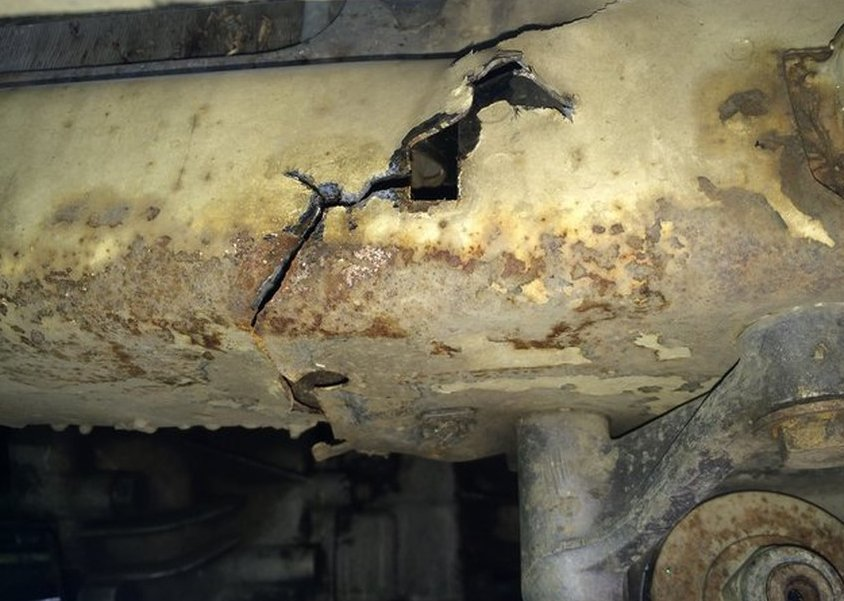
\includegraphics[width=.49\textwidth]{images/tc5}
  		\caption{\footnotesize {Повреждение левой нижней части панели рамки радиатора  }}
  		\label{ris:images/tc5}}
  	\hfil \hfil
  	\parbox[t]{0.49\textwidth}
  	{\centering
  		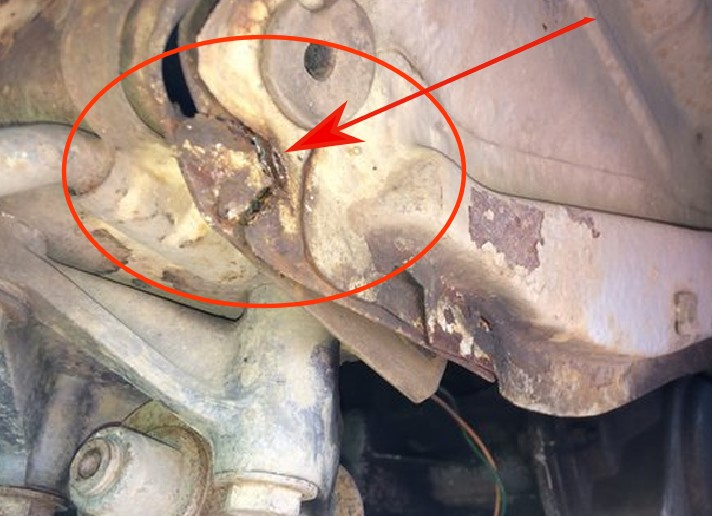
\includegraphics[width=.49\textwidth]{images/tc4}
  		\caption{\footnotesize {Повреждение передней нижней части левого лонжерона}}
  		\label{ris:images/tc4}}
  \end{figure}
%%%%%%%%%%%%%%%%%%%%%%%%%%%%%%%%%%%%%%%%%%%  

\begin{figure}[h]
	\centering
	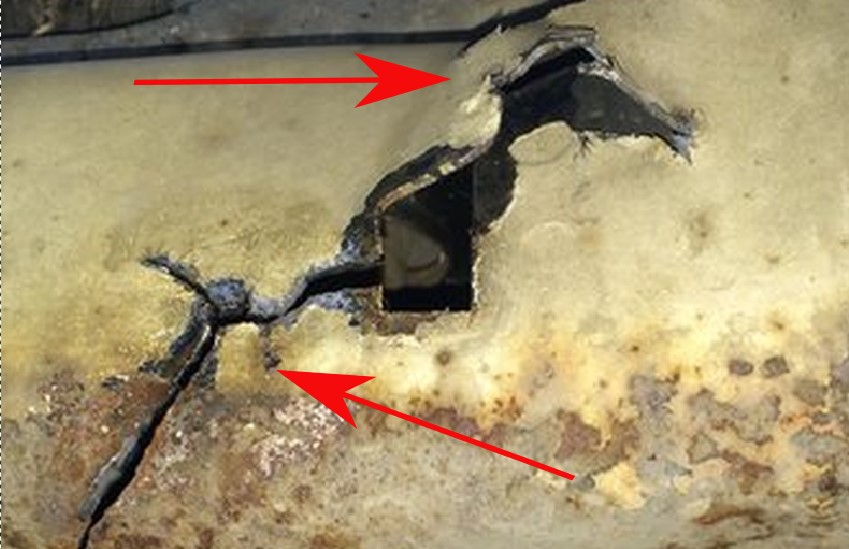
\includegraphics[width=0.98\linewidth]{images/tc6}
	\caption{{\footnotesize {Разрыв панели рамки радиатора внизу слева. Вид спереди}}}
	\label{ris:images/tc6}
\end{figure}
\pagebreak

\begin{figure}[!h]
	\centering
	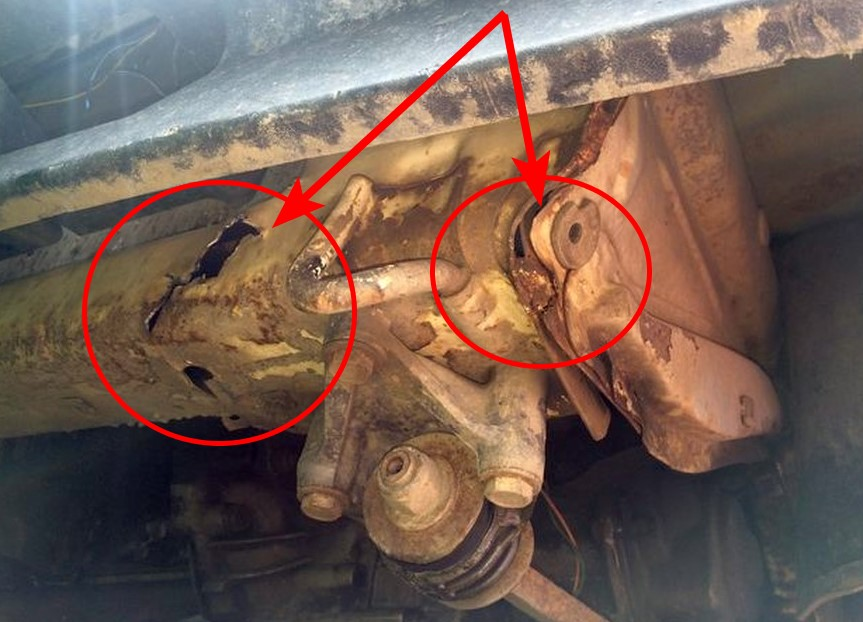
\includegraphics[width=0.98\linewidth]{images/tc7}
	\caption{{\footnotesize {Разрыв панели рамки радиатора внизу слева. Вид снизу слева. "1" - }}}
	\label{ris:images/tc7}
\end{figure}

\begin{figure}[!h]
	\centering
	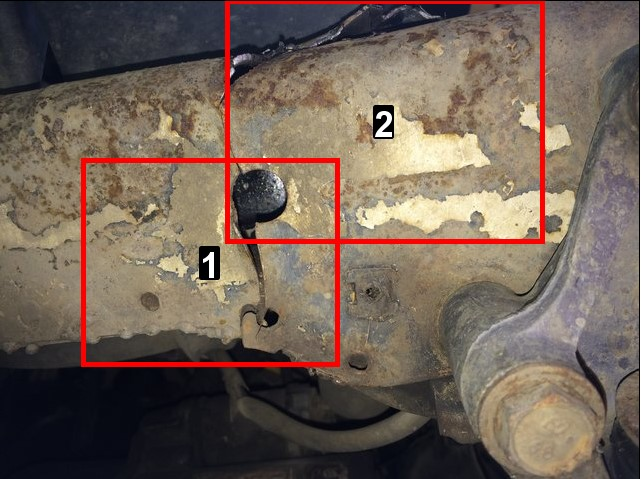
\includegraphics[width=0.98\linewidth]{images/tc11}
	\caption{{\footnotesize {Разрыв панели рамки радиатора внизу слева. Вид снизу слева}}}
	\label{ris:images/tc11}
\end{figure}

\begin{figure}[H]
	\centering
	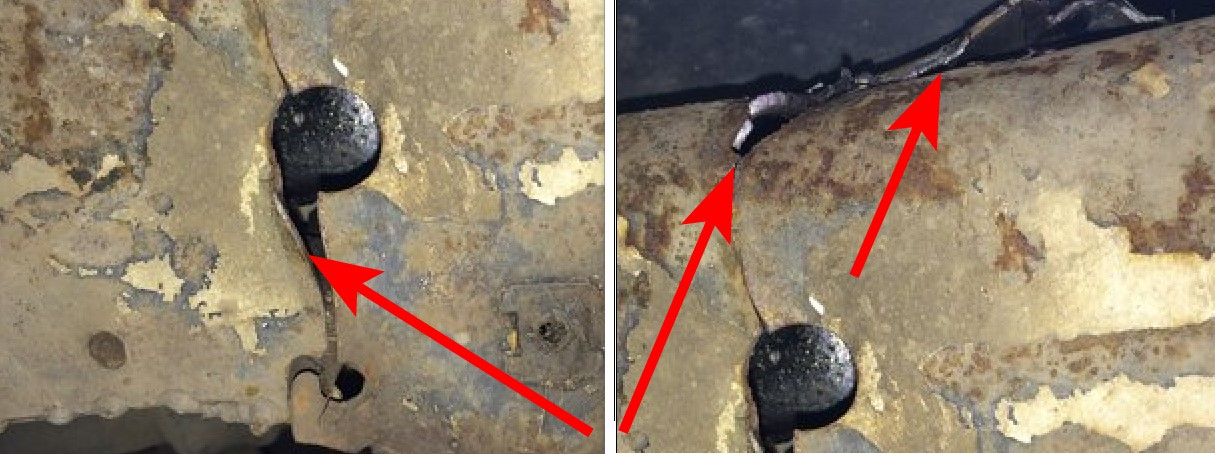
\includegraphics[width=0.98\linewidth]{images/tc12}
	\caption{{\footnotesize {Разрыв панели рамки радиатора. Слева усталостные трещины, справа - деформация и разрыв}}}
	\label{ris:images/tc12}
\end{figure}


Анализ поверхностных  деформаций крыла переднего левого  автомобиля \тс\, показывает, что в процессе столкновения  автомобиль \тс\, находился в движении по направлению "вперед", так как  относительно продольной оси автомобиля \тс\,, вектор удара направлен слева направо и спереди назад, автомобиль Renault Master мог двигаться в направлении слева направо, пересекая траекторию движения \тс, Таким образом, согласно имеющимся материалам, механизм столкновения,    вероятно, соответствует перекрестному, косому, скользящему, эксцентричному, левому столкновению.  Ударное воздействие локализовалось в области левой передней стойки автомобиля, при этом крыло переднее левое деформировалось на глубину не менее 5см, передняя  кромка двери левой передней получила загиб на глубину не менее 3 см в направлении действия сил, верхняя петля и примыкающая к ней часть левой передней стойки так же получили деформацию.  

Из технических данных  цифровых изображений EXIF известно, что 
фотографирование поврежденного автомобиля производилось  2016:07:19 в 14:44:54,  согласно справки о дорожно-транспортном происшествии, ДТП произошло 2016:07:19 в 13:42 то есть через 1 час после заявленного страхового события. Актом осмотра № 295, л.д. 19, составленным ИП Новиковым О.Н. 19.07.2016г. зафиксировано, в том числе, повреждение панели рамки радиатора слева и брызговик с лонжероном  слева.

На фотоизображениях Рис. \ref{ris:images/tc11} и Рис. \ref{ris:images/tc12} эксперт обращает внимание на два различающихся внешними признаками  вида повреждений ( области "1" и "2"). Повреждения, отмеченные на Рис. \ref{ris:images/tc11} выделенной областью "1" и левый снимок на Рис. \ref{ris:images/tc12} имеют характерные для усталостного разрушения трещины металла, возникающие под воздействием знакопеременной нагрузки или периодической динамической нагрузки. Коррозия поверхности излома металла в нижней части балки однозначно указывают на повреждение, образовавшееся задолго до дорожно-транспортного происшествия \датадтп.  Повреждения, отмеченные областью "2", правый снимок на Рис.  \ref{ris:images/tc12} и на Рис.\ref{ris:images/tc6}  имеют характер пластической деформации с разрывом металла, при этом, поверхности металла на разрыве имеют чистый металлический цвет без загрязнений и следов коррозии. Совокупность морфологических признаков этой части повреждений нижней поперечины рамки радиатора позволяют эксперту полагать, что указанные повреждения могут являться вторичными деформациями вследствие ДТП от \датадтп.

 \begin{figure}[H]
 	\centering
 	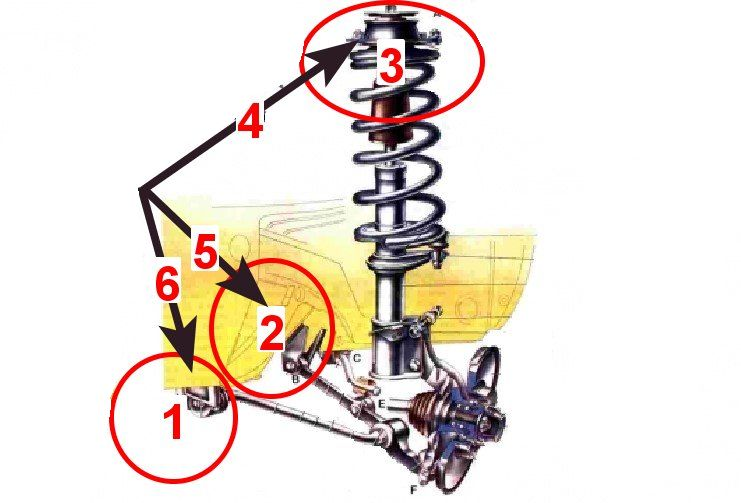
\includegraphics[width=0.75\linewidth]{images/s1}
 	\caption{{\footnotesize {Cхема деталей передней подвески ВАЗ 21099}}}
 	\label{ris:images/s1}
 \end{figure}

На Рис.\ref{ris:images/s1} приведена схема передней подвески автомобилей ВАЗ 21099, на которой стрелками показаны точки крепления подвески к кузову автомобиля.  Стрелка 6 указывает на область 1, где расположено крепление продольной растяжки к нижней поперечине рамки радиатора, стрелка 5 указывает на  область 2, место крепление поперечного рычага к основанию лонжерона и стрелка 4 указывает на точку 3 - место крепления стойки передней подвески к брызговику. Крепление рычага, растяжки и стойки выполнено через сайлентблоки. Практика ремонта автомобилей ВАЗ 2108-2109 показывает, что участок места крепления кронштейна рычага к панели рамки радиатора (на схеме отмечен "1"), в силу конструктивных особенностей, является  концентратором напряжений. 

 \begin{figure}[H]
	\centering
	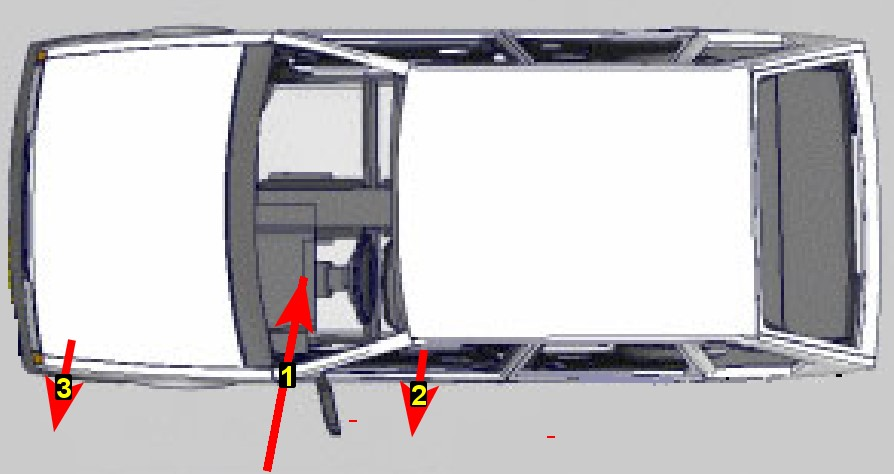
\includegraphics[width=0.75\linewidth]{images/s2}
	\caption{{\footnotesize {Направление   ударного воздействия  и реакции кузова ВАЗ 2109}}}
	\label{ris:images/s2}
\end{figure}

На рисунке \ref{ris:images/s2}  стрелка 1 показывает направление  вектора удара, стрелки 2 и 3 направление реакции кузова.

\pagebreak

\begin{multicols}{3}[\columnsep=1cm]
\noindent	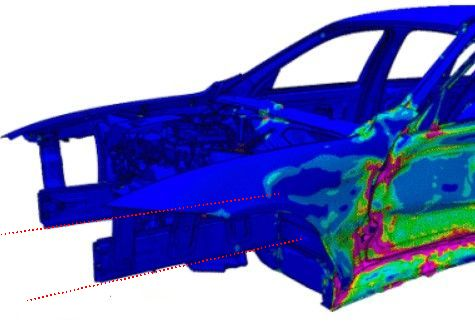
\includegraphics[scale=0.5]{m1}
	\columnbreak
	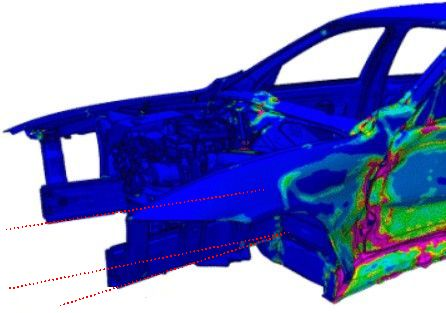
\includegraphics[scale=0.5]{m2}
	\columnbreak
	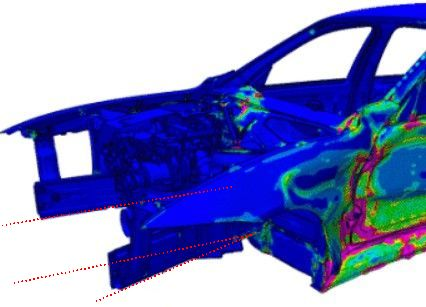
\includegraphics[scale=0.5]{m3}
\end{multicols}


\captionof{figure}{\footnotesize{Пример конечно-элементной модели реакции кузова автомобиля при боковом ударе (по материалам CompMechLab LLC, \url{http://fea.ru/compound/automotive}  ) }}

  \vspace{3mm}

На примере конечно-элементной модели автомобиля  наглядно видно, что при  ударном воздействии в боковую стойку в направлении слева направо левый передний лонжерон стремиться сместится в направлении, противоположном вектору удара. При этом, отклонение лонжерона от продольной оси может составлять нескольких сантиметров. Таким образом, именно в области левой нижней части панели рамки радиатора автомобиля \тс в месте сопряжения с передним левым лонжероном при боковом ударе создается дополнительная  концентрация напряжений.

 В случае исследуемого ДТП, имело место  сочетание ослабления места крепления кронштейна  рычага на панели рамки радиатора вследствие  усталости металла и образования дополнительной концентрации напряжений, возникшей в результате ударной нагрузки в область передней левой стойки автомобиля, что, в совокупности, привело к превышению предела прочности и  разрушению панели раки радиатора и передней нижней части левого лонжерона.  

\section{Вывод} 


\textbf{  <<Повреждение панели рамки радиатора слева и брызговика с лонжероном переднего левого автомобиля ВАЗ 21099 связано  с указанным ДТП.>>	}
  
  
  \vspace{20mm}
{Эксперт}\hfill           {Алифиренко В.В.}


